\documentclass[12pt,a4paper]{article}
\usepackage[T1,T2A]{fontenc}
\usepackage[utf8]{inputenc}
\usepackage[english,russian]{babel}
\usepackage{microtype}
\usepackage{csquotes}
\usepackage{amsmath}
\usepackage{amsthm}
\usepackage{amssymb}
\usepackage{mathtext}
\usepackage{newfloat}
\usepackage{caption}
\usepackage{indentfirst}
\usepackage{geometry}
\usepackage{hyperref}
\usepackage{mdframed}
\usepackage[inline]{enumitem}
\usepackage{graphicx}
\usepackage{subfig}
\DeclareGraphicsExtensions{.pdf,.png,.jpg,.PNG}
\graphicspath{{./img/}}
\captionsetup[figure]{justification=centering}
\renewcommand{\thesubfigure}{\asbuk{subfigure}}
\DeclareCaptionLabelSeparator{dotseparator}{. }
\captionsetup{
   labelsep=dotseparator
}

\begin{document}

\section{Постановка задачи}

Исследовать поведение электрона в скрещенных электрическом и магнитном статических полях.

\section{Физическая модель}

Будем полагать, что электрон -- точечный заряд, находящийся в пустом однородном изотропном пространстве. В том же пространстве существуют постоянные во времени однородные электрическое и магнитное поле. Рассматривается нерелятивистский случай.

\section{Математическая модель}

Для вывода закона движения электрона воспользуемся ньютоновской динамикой.

Известно, что силу, действующую на точечный заряд со стороны электромагнитного поля, можно представить в виде
%%
\begin{equation}
\vec{F}_{em} = q \vec{E} + q \left[\vec{v} \times \vec{B}\right] \textrm{,}
\end{equation}
%%
где первый член отражает вклад силы, действующей со стороны электрического, а второй -- магнитного поля.

Для решаемой задачи справедливо
%%
\begin{equation} \label{eq:pre_motion_law}
m \vec{a} = \vec{F}_{em} \textrm{.}
\end{equation}

Поделив \autoref{eq:pre_motion_law} на $m$, получим в итоге закон движения электрона:
%%
\begin{equation} \label{eq:motion_law}
\ddot{\vec{r}} = \frac{q}{m} \vec{E} + \frac{q}{m} \left[\dot{\vec{r}} \times \vec{B}\right] \textrm{.}
\end{equation}
%%

\section{Численная модель}

В целях борьбы с погрешностями, вносимыми спецификой компьютерных вычислений, проведем обезразмеривание параметров закона движения.

Положим
%%
\begin{equation} \label{eq:let}
\vec{e} = \frac{q}{m} \frac{\vec{E}}{e_0}       \quad %
\vec{b} = \frac{q}{m} \frac{\vec{B}}{b_0}       \quad %
\vec{u} = \frac{\vec{v}}{u_0}                   \textrm{.}
\end{equation}
%%

Тогда, подставляя \autoref{eq:let} в \autoref{eq:motion_law} и деля на $u_0$, а также вводя
%%
\begin{equation}
\dot{\vec{r}} = \vec{v} = u_0 \vec{u} \textrm{,}
\end{equation}
%%
получим
%%
\begin{equation}
\dot{\vec{u}} = \frac{e_0}{u_0} \vec{e} + b_0 \left[\vec{u} \times \vec{b}\right] \textrm{.}
\end{equation}

Получившаяся система обыкновенных дифференциальных уравнений первого порядка при заданных начальных условиях ($\vec{r}(0) = \vec{r}_0 \textrm{, } \vec{v}(0) = \vec{v}_0$) может быть решена методом Рунге-Кутты 4-го порядка.

Для простоты при моделировании будем использовать постоянный шаг по времени. Без потери общности положим $\vec{r_0} = 0$. Из дальнейших исследований видно, что нормировочные параметры $u_0$, $e_0$ и $b_0$ могут быть выбраны равными единице.

\section{Результаты и их обсуждение}

В ходе работы была написана демонстрационная программа на языке $c++$. Программа позволяет исследовать движение электрона по графикам $\vec{r}(t)$ и $r_i(r_j)$ в зависимости от конфигурации полей и начальной скорости.

Внешний вид программы приведен на \autoref{fig:mainwindow}.

\begin{figure}[h]%
\centering
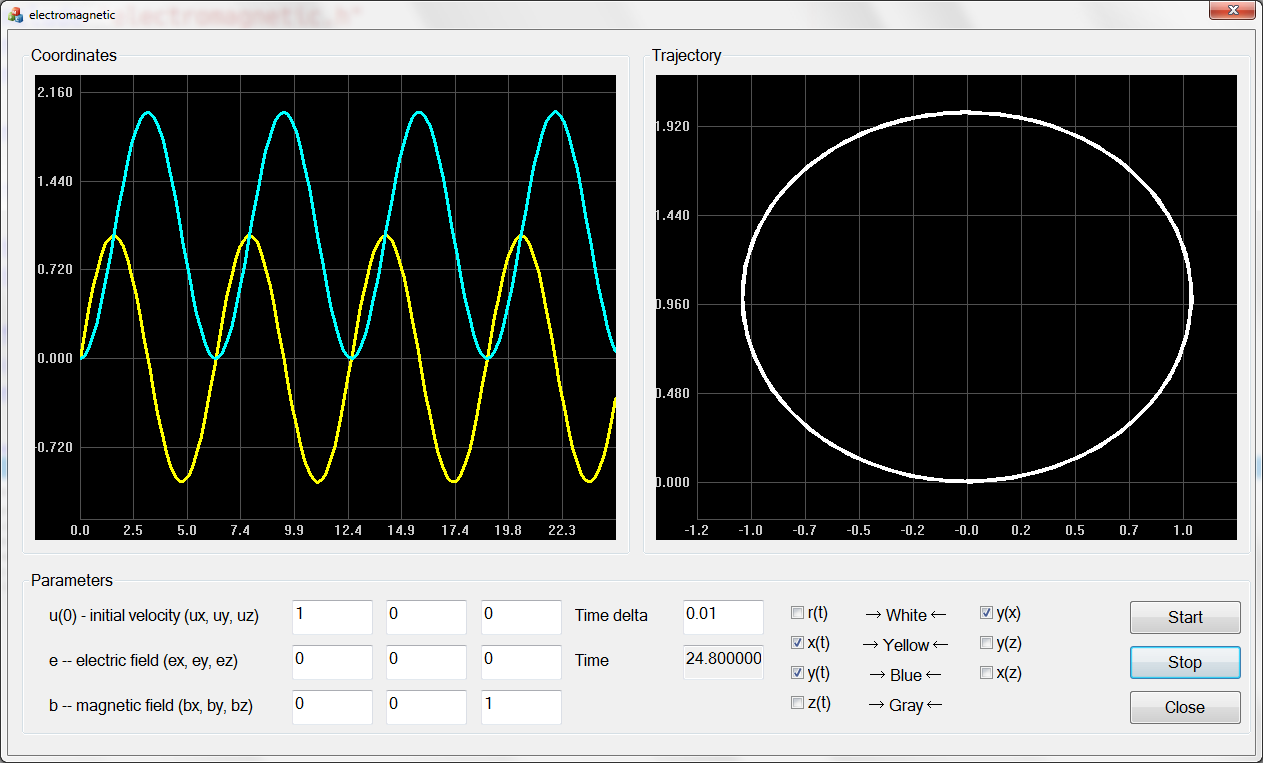
\includegraphics[width=0.8\textwidth]{mainwindow}%
\caption[Главное окно программы.]{Главное окно программы}%
\label{fig:mainwindow}%
\end{figure}

В левой области отображаются временн\`{ы}е зависимости. В правой -- траектории в различных сечениях ($y(x)$, $y(z)$, $x(z)$). По осям графиков откладываются величины $t$ и $r_i$. Проекции полей вводятся в единицах отношения $e / m_e$ заряда электрона к его массе.

Рассмотрим результат моделирования нескольких классических случаев.

\subsection{Движение в электрическом поле в плоскости $OXY$}

Задача полностью эквивалентна баллистической задаче о движении тела в поле тяжести, брошенного под углом к горизонту. Роль силы тяжести здесь выполняет произведение заряда на напряженность электрического поля, взятую с противоположным знаком. Результат моделирования представлен на \autoref{fig:electric}.

\begin{figure}[h]%
\centering
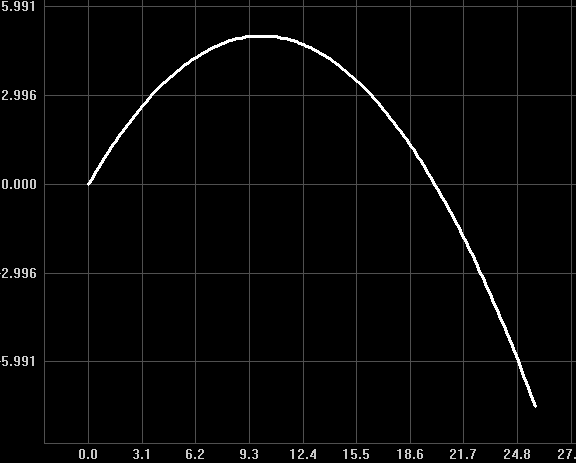
\includegraphics[width=0.8\textwidth]{electric}%
\caption[Движение в электрическом поле]{Движение в электрическом поле при наличии двух проекций у начальной скорости. Электрическое поле направлено по оси $OY$}%
\label{fig:electric}%
\end{figure}

\subsection{Движение в магнитном поле в плоскости $OXY$}

Пусть в пространстве существует только магнитное поле. В этом случае на заряд будет действовать только сила со стороны магнитного поля, причем ее направление в любой момент времени перпендикулярно плоскости, образованной $\vec{u}(t)$ и $\vec{b}$.

Рассмотрим заряд, влетающий в магнитное поле так, что $\vec{u}(0)\ \bot\ \vec{b}$. Очевидно, что заряд будет двигаться в плоскости, перпендикулярной вектору $\vec{b}$, причем, т.к. на него действует одинаковая по модулю сила, всегда направленная перпендикулярно скорости его движения, траекторией будет окружность (\autoref{fig:magnetic}).

Если у заряда также имеется составляющая скорости вдоль поля $\vec{b}$, то движение будет происходить по винтовой линии (\autoref{fig:magnetic_vz}). Картина в перпендикулярной полю плоскости не изменится.

\begin{figure}[h]%
\centering
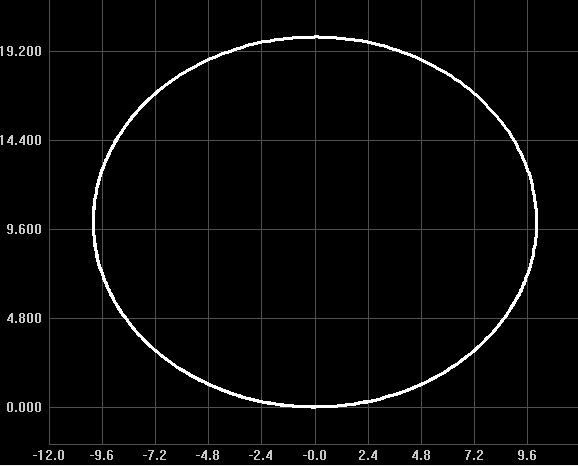
\includegraphics[width=0.8\textwidth]{magnetic}%
\caption[Движение в магнитном поле]{Движение в магнитном поле. Начальная скорость направлена по оси $OX$. Магнитное поле направлено по оси $OZ$}%
\label{fig:magnetic}%
\end{figure}

\begin{figure}[h]%
\centering
%
\subfloat[][]{%
\label{fig:magnetic_x_of_z}%
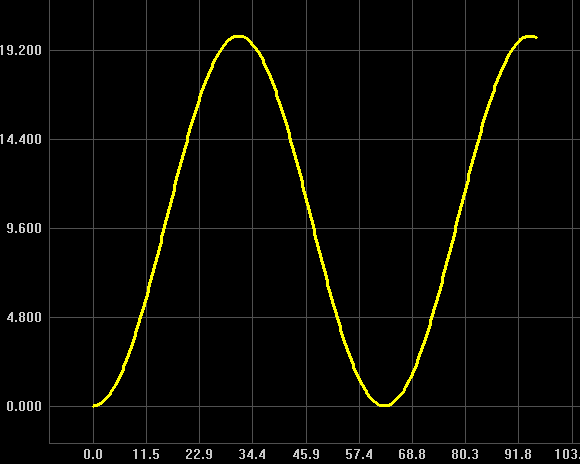
\includegraphics[width=0.4\textwidth]{magnetic_x_of_z}}%
\hspace{8pt}%
%
\subfloat[][]{%
\label{fig:magnetic_y_of_z}%
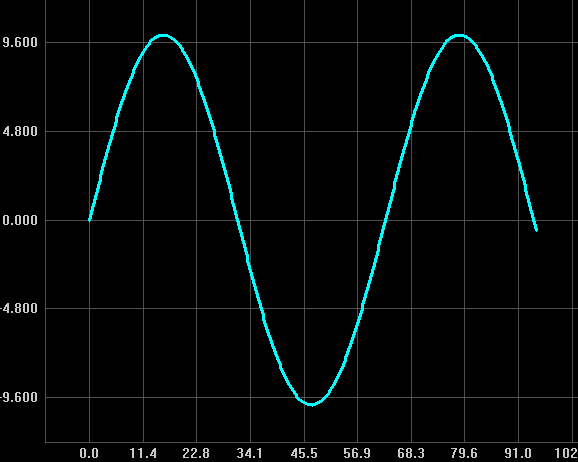
\includegraphics[width=0.4\textwidth]{magnetic_y_of_z}}%
\hspace{8pt}%
%
\caption[Движение в магнитном поле]{Движение в магнитном поле. Начальная скорость имеет проекции на оси $OX$ и $OZ$. Магнитное поле направлено по оси $OZ$.
\subref{fig:magnetic_x_of_z} $x(z)$ %
\subref{fig:magnetic_y_of_z} $y(z)$} %
\label{fig:magnetic_vz}%
\end{figure}

\subsection{Движение в перпендикулярных электрическом и магнитном полях}

При совместном действии электрического и магнитного поля решение задачи усложняется.

Случай $\vec{e}\ ||\ \vec{b}$ не интересен к рассмотрению, поскольку является простой суперпозицией предыдущих двух: заряд будет ускоренно двигаться по винтовой линии.

Рассмотрим случай, когда $\vec{e}\ \bot\ \vec{b}$. Сила со стороны магнитного поля будет действовать в той же плоскости, что и сила со стороны электрического поля. Не сложно показать, что траекторией заряда будет являться циклоида, что и наблюдается при моделировании (\autoref{fig:electromagnetic}).

\begin{figure}[h]%
\centering
%
\subfloat[][]{%
\label{fig:electromagnetic_1}%
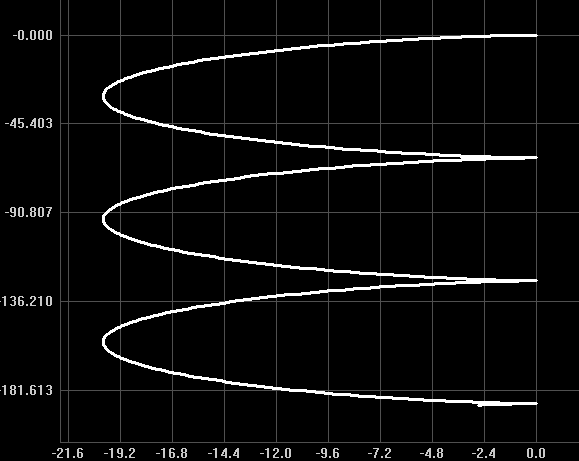
\includegraphics[width=0.3\textwidth]{electromagnetic_1}}%
\hspace{8pt}%
%
\subfloat[][]{%
\label{fig:electromagnetic_2}%
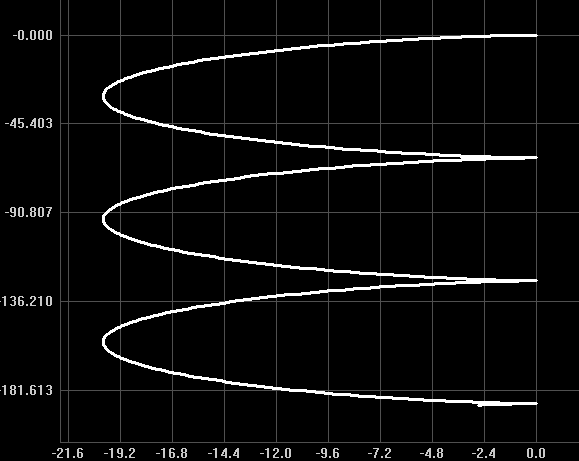
\includegraphics[width=0.3\textwidth]{electromagnetic_1}}%
\hspace{8pt}%
%
\subfloat[][]{%
\label{fig:electromagnetic_3}%
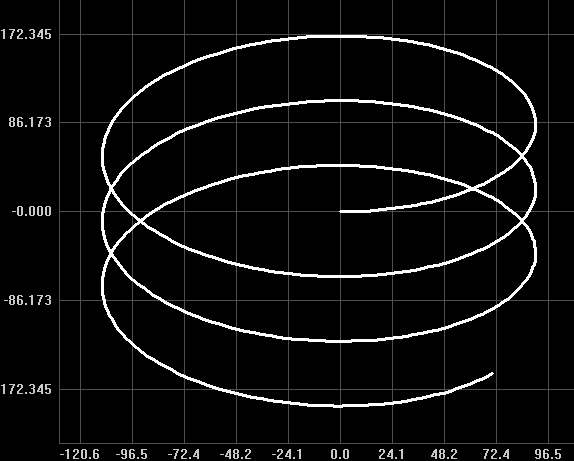
\includegraphics[width=0.3\textwidth]{electromagnetic_3}}%
\hspace{8pt}%
%
\caption[Движение в электромагнитном поле]{Движение в электромагнитном поле. Магнитное поле направлено по оси $OZ$. Электрическое поле направлено по оси $OX$.
\subref{fig:electromagnetic_1} без начальной скорости %
\subref{fig:electromagnetic_2} с начальной скоростью вдоль оси $OX$ %
\subref{fig:electromagnetic_3} с большей по модулю начальной скоростью вдоль оси $OX$} %
\label{fig:electromagnetic}%
\end{figure}

\section{Выводы}

В ходе работы была написана демонстрационная программа для исследования поведения электрона в скрещенных электрическом и магнитном полях.

Были проанализированы несколько характерных для задачи случаев, а именно движение отдельно в электрическом, отдельно в магнитном и одновременно во взаимно перпендикулярных электрическом и магнитном полях.

Были получены графики траекторий движения частицы для рассмотренных случаев. Графики согласуются с известными из теоретического анализа фактами.

\end{document} 